%iffalse
\let\negmedspace\undefined
\let\negthickspace\undefined
\documentclass[journal,12pt,onecolumn]{IEEEtran}
\usepackage{cite}
\usepackage{amsmath,amssymb,amsfonts,amsthm}
\usepackage{algorithmic}
\usepackage{graphicx}
\usepackage{textcomp}
\usepackage{xcolor}
\usepackage{txfonts}
\usepackage{listings}
\usepackage{enumitem}
\usepackage{mathtools}
\usepackage{gensymb}
\usepackage{comment}
\usepackage[breaklinks=true]{hyperref}
\usepackage{tkz-euclide} 
\usepackage{listings}
\usepackage{gvv}                                        
%\def\inputGnumericTable{}                                 
\usepackage[latin1]{inputenc}                                
\usepackage{color}                                            
\usepackage{array}                                            
\usepackage{longtable}                                       
\usepackage{calc}                                             
\usepackage{multirow}                                         
\usepackage{hhline}                                           
\usepackage{ifthen}                                           
\usepackage{lscape}
\usepackage{tabularx}
\usepackage{array}
\usepackage{float}
\usepackage{multicol}
\usepackage{subcaption}

\newtheorem{theorem}{Theorem}[section]
\newtheorem{problem}{Problem}
\newtheorem{proposition}{Proposition}[section]
\newtheorem{lemma}{Lemma}[section]
\newtheorem{corollary}[theorem]{Corollary}
\newtheorem{example}{Example}[section]
\newtheorem{definition}[problem]{Definition}
\newcommand{\BEQA}{\begin{eqnarray}}
\newcommand{\EEQA}{\end{eqnarray}}
\newcommand{\define}{\stackrel{\triangle}{=}}
\theoremstyle{remark}
\newtheorem{rem}{Remark}


% Marks the beginning of the document
\begin{document}
\bibliographystyle{IEEEtran}
\vspace{3cm}

\title{NCERT-12.8.1.4}
\author{S. Sai Akshita - EE24BTECH11054}
\newpage
\maketitle
\bigskip

\renewcommand{\thefigure}{\theenumi}
\renewcommand{\thetable}{\theenumi}
\textbf{Question:} Find the area of the region bounded by the ellipse
\begin{align}
\frac{x^2}{16}+\frac{y^2}{9}=1. \label{eq.1}
\end{align}
\textbf{Obtaining solution using Integration(Theoretical):}

Rewriting the equation for $ y $:
\begin{align}
y = \pm \frac{3}{4} \sqrt{16 - x^2} \label{eq.2}
\end{align}

The total area of the ellipse can be computed as:
\begin{align}
A = \int_{-4}^{4} 2y \, dx
\end{align}

Substituting \ref{eq.2}, the area becomes:
\begin{align}
A = 2 \int_{-4}^{4} \frac{3}{4} \sqrt{16 - x^2} \, dx
\end{align}

Simplifying:
\begin{align}
A = \frac{3}{2} \int_{-4}^{4} \sqrt{16 - x^2} \, dx
\end{align}
Due to the symmetry of the ellipse, we can calculate the area over the interval $\sbrak{0,4}$ and multiply it by 2:
\begin{align}
A &= 2 \times \frac{3}{2} \int_{0}^{4} \sqrt{16 - x^2} \, dx\\
A &= 3 \int_{0}^{4} \sqrt{16 - x^2} \, dx\\
A &= 3\times\frac{1}{2}\sbrak{x\sqrt{16-x^2}+16\sin^{-1}\brak{\frac{x}{4}}  }\Biggr|_{0}^{4}\\
A &= 12\pi \approx 37.699
\end{align}
\textbf{Numerical Integration Using the Trapezoidal Rule(simulation):}\\
Trapezoidal Rule is a rule that evaluates the area under the curves by dividing the total area into smaller trapezoids rather than using rectangles. This integration works by approximating the region under the graph of a function as a trapezoid, and it calculates the area.\\
The integral:
\begin{align}
\int_{0}^{4} \frac{3}{4}\sqrt{16 - x^2} \, dx
\end{align}
can be approximated using the Trapezoidal Rule.\\
\textbf{The Trapezoidal Rule formula:}
\begin{align}
\int_a^b f\brak{x} \, dx \approx \frac{h}{2} \sbrak{ f\brak{x_0} + 2 \sum_{k=1}^{n-1} f\brak{x_k} + f\brak{x_n} }\label{eq.3}
\end{align}
where:
\begin{align}
h = \frac{b - a}{n}, \quad x_k = a + k h \quad \text{for } k = 0, 1, \dots, n
\end{align}
But we already know that
For the ellipse:
\begin{align}
f\brak{x} = \frac{3}{4}\sqrt{16 - x^2}, \quad a = 0, \quad b = 4
\end{align}
This formula \ref{eq.3} is derived by the sum of areas of all the trapezoids fitted under the curve.
Using $n$ subintervals, we should compute the values $ x_k = a + kh $ and $ y_k=f\brak{x_k} = \frac{3}{4}\sqrt{16 - x_k^2} $.\\ Then, we can apply the Trapezoidal Rule formula to approximate the integral by simulation.\\
By differentiating \ref{eq.1}, we get
\begin{align}
    \frac{dy}{dx}&=\frac{-9x}{16y} \label{eq.4}\\
\end{align}
Forming difference equation for simulation from \ref{eq.4}:
\begin{align}
x_{n+1}&=x_n+h\\
    y_{n+1}&=y_n+h\brak{\frac{-9x_n}{16y_n}}\\
\end{align}
By using above equations, we can find the area of $n^{th}$ trapezoid inside the curve.
By opting proper value of $n$, we can form $n$ trapezoids by using the difference equation under the curve. The bigger the value of $n$, the lesser the error of the obtained area value will be.
  

\begin{figure}[htbp] 
    \centering % Center the figure
    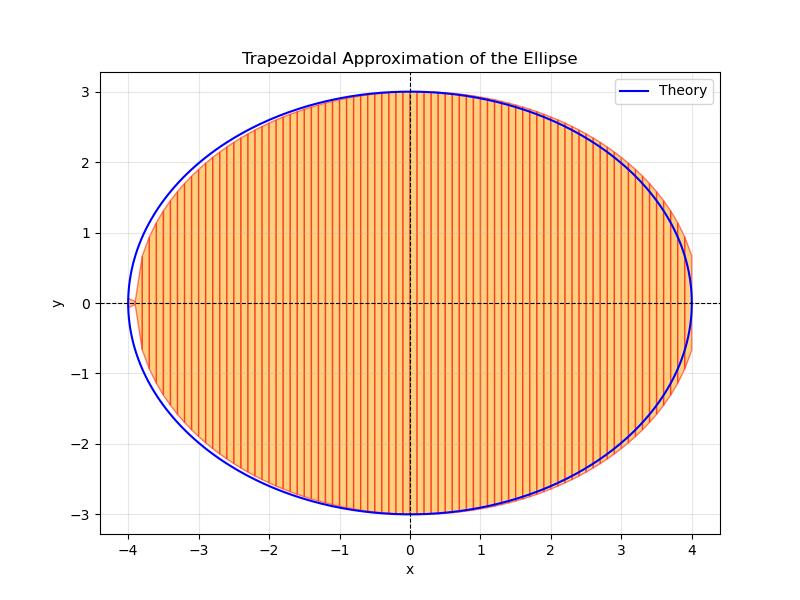
\includegraphics[width=\linewidth]{Theory and sim.jpeg} 
    \label{fig:example} % Label for referencing in text
\end{figure}


   
\end{document}
